\documentclass{bbawslides}

\usepackage[TS1, T1]{fontenc}
\usepackage{ifthen}

\usepackage[a4paper]{hyperref}
\rotateheaderstrue	%%-- otherwise seminar does strange things
\usepackage{url}

\usepackage[ngerman]{babel}
\usepackage[babel]{csquotes}
\usepackage[autoplay]{animate}
\usepackage{graphicx}
\usepackage{numprint}
\usepackage{multicol}
\npthousandsep{~}\npthousandthpartsep{}\npdecimalsign{,}

\DeclareTextSymbol{\textlongs}{TS1}{115} 
\DeclareTextSymbolDefault{\textlongs}{TS1}


\begin{document}
\providecommand{\Title}{}


\begin{bbawtitle}[Perspektiven der automatischen Texterfassung als Grundlage
wissenschaftlicher Editionen]
  \vspace*{0.5em}%
  \textcolor{bbawred}{\bf am Beispiel der Brief- und Schriftenausgabe\\der \textsc{Bernd Alois Zimmermann}-Gesamtausgabe}\\[4ex]
  %Matthias Boenig, Hemma Jäger, Matthias Pasdzierny, Kay-Michael Würzner\\[-.25em]%
  %\textcolor{urlColor}{\texttt{{\small \{boenig|hemma.jaeger|pasdzierny|wuerzner\}@bbaw.de}}}
  Matthias Boenig \& Kay-Michael Würzner\\[-.25em]%
  \textcolor{urlColor}{\texttt{{\small \{boenig|wuerzner\}@bbaw.de}}}
  \\[1.5em]
  {\scriptsize{%
    Geisteswissenschaftliche Forschungsdaten.\\Methoden zur digitalen Erfassung, Aufbereitung und Präsentation\\%
    19. Oktober 2017\\%
  }}
\end{bbawtitle}
\slideStyleFrame

\renewcommand{\footerText}{\tiny 19. Oktober 2017, Workshop AG eHumanities}

%----------------------------------------------------------------------------------------------
% Outline
%----------------------------------------------------------------------------------------------
\begin{bbawslide}{Übersicht}
  \vspace*{7mm}%
  \centerslidestrue%
  \begin{itemize}
    \item Einleitung
    \begin{itemize}\small
      \item die \textsc{Bernd Alois Zimmermann}-Gesamtausgabe
      \item Motivation
      \item automatische Texterfassung
    \end{itemize}
    \item Workflowbeschreibung
    \begin{itemize}\small
      \item Bildvorverarbeitung
      \item Layoutanalyse
      \item Zeichenerkennung
      \item Textbearbeitung
    \end{itemize}
    \item Perspektiven
    \begin{itemize}\small
      \item Volltextverbesserung
      \item OCR-D
      \item Editionsunterstützung
    \end{itemize}
  \end{itemize}
\end{bbawslide}

\begin{bbawpart}{\Large\bf Einleitung}
\end{bbawpart}

\begin{bbawslide}{Die \textsc{Bernd Alois Zimmermann}-Gesamtausgabe}
  \vspace*{7mm}%
  \centerslidestrue%
  \begin{itemize}
    \item gemeinsames \textbf{Langzeitvorhaben} der Akademien in Mainz und Berlin
    \item jüngste musikwissenschaftliche Gesamtausgabe
    \item Ziele:
    \begin{itemize}
      \item Edition der Kompositionen
      \item Herausgabe der \textbf{Schriften} und \textbf{repräsentativer Teile} der Korrespondenz (\enquote{Spiegel der breiteren Debattengeschichte der zweiten Hälfte\\des 20. Jh.})
    \end{itemize}
    \item Anwendung computergestützter Methoden bei \textbf{Erfassung} und Auswertung
    \item bisher ca. 6000 Objektseiten in der Abteilung Schriften und Briefe digitalisiert
  \end{itemize}
\end{bbawslide}

\begin{bbawslide}{Die \textsc{Bernd Alois Zimmermann}-Gesamtausgabe}
  \vspace*{3mm}%
  \centerslidestrue%
  \textbf{Beispiele:}
  \begin{center}
    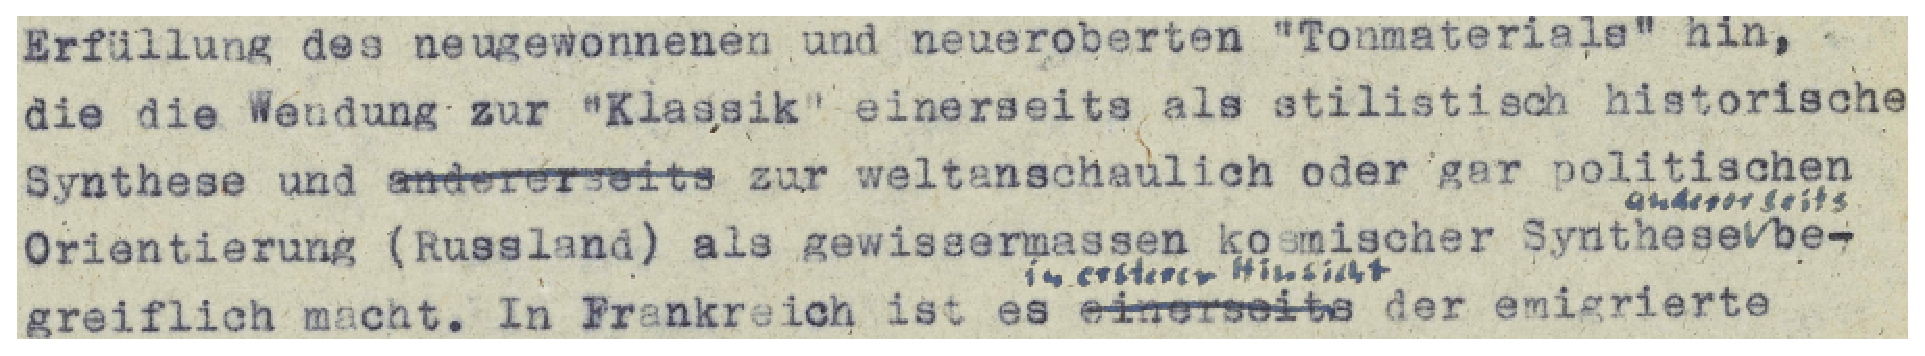
\epsfig{file=figures/ex_typo1.eps,width=\textwidth}
    \begin{tabular}{cc}
      \begin{minipage}{0.3\textwidth}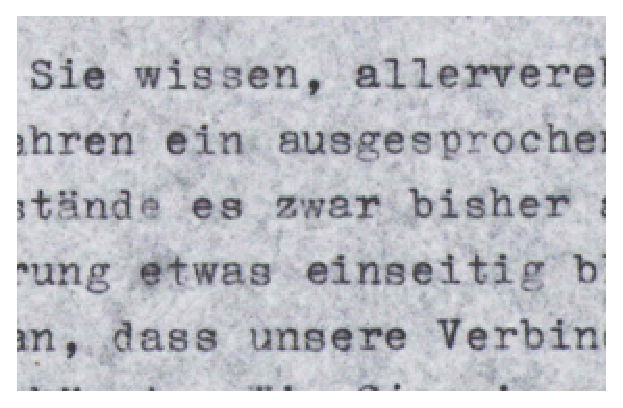
\epsfig{file=figures/ex_typo2.eps,width=\textwidth}\end{minipage}
      &
      \begin{minipage}{0.3\textwidth}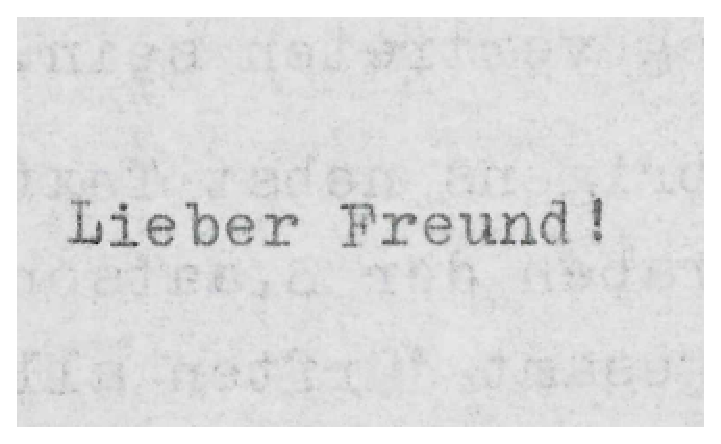
\epsfig{file=figures/ex_typo3.eps,width=\textwidth}\end{minipage}
    \end{tabular}
    \begin{tabular}{cc}
      \begin{minipage}{0.3\textwidth}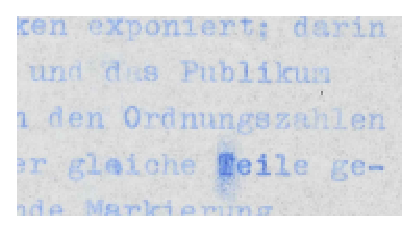
\epsfig{file=figures/ex_typo4.eps,width=\textwidth}\end{minipage}
      &
      \begin{minipage}{0.3\textwidth}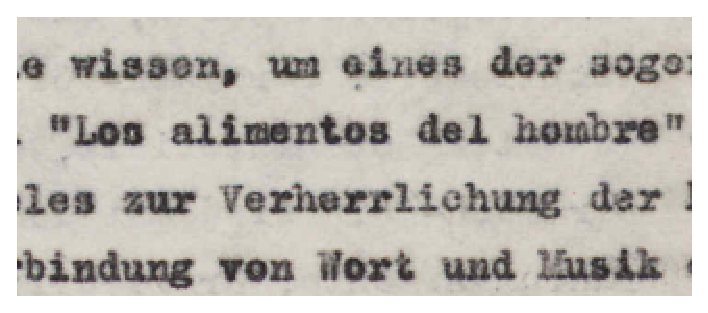
\epsfig{file=figures/ex_typo5.eps,width=\textwidth}\end{minipage}
    \end{tabular}
  \end{center}
\end{bbawslide}

\begin{bbawslide}{Motivation}
  \vspace*{7mm}%
  \centerslidestrue%
  \begin{itemize}
    \item \textbf{Pilotstudie} zum Einsatz von automatischer Texterfassung zur Editionsvorbereitung
    \item Kooperation der \textsc{Bernd Alois Zimmermann}-Gesamtausgabe mit OCR-D (DFG-Koordinationsprojekt zur Verbesserung von OCR-Verfahren)
    \item Fragestellungen:
    \begin{enumerate}
      \item Vorteile grundständig \textbf{manueller Erfassung vs. automatischer Erfassung} mit anschließender Expertenbearbeitung
      \item \textbf{Einfluss} der opportunistischen Texterfassung (vs. vorausgehender gezielter Textauswahl) \textbf{auf den Editionsprozess}
    \end{enumerate}
  \end{itemize}
\end{bbawslide}

\begin{bbawslide}{Automatische Texterfassung}
  \vspace*{7mm}%
  \hspace*{-2.5em}%
  \centerslidestrue%
  \begin{tabular}{lc}
    \begin{minipage}{0.65\textwidth}
      \begin{itemize}
        \item Textquellen mehrheitlich nicht in \emph{digitaler} Form verfügbar
        \begin{itemize}\small
          \item historische Bücher, Zeitungen und andere Druckerzeugnisse
          \item handgeschriebene Manuskripte und Briefe
        \end{itemize}
        \item Bewahrung/Konservierung durch Scan oder Foto
        \begin{itemize}\small
          \item Bilder sind \textbf{kein Text}
          \item[\textcolor{bbawred}{$\Rightarrow$}] Textsuche oder quantitative Auswertung nicht möglich
        \end{itemize}
        \item Automatische Erfassung von \textbf{Text} in Bildern (aka.~\textbf{O}ptical \textbf{C}haracter \textbf{R}ecognition)
        \item Automatische Erfassung des \textbf{Layouts} in Bildern (aka.~\textbf{O}ptical \textbf{L}ayout \textbf{R}ecognition)
      \end{itemize}
    \end{minipage}
    &
    \begin{minipage}{0.4\textwidth}
        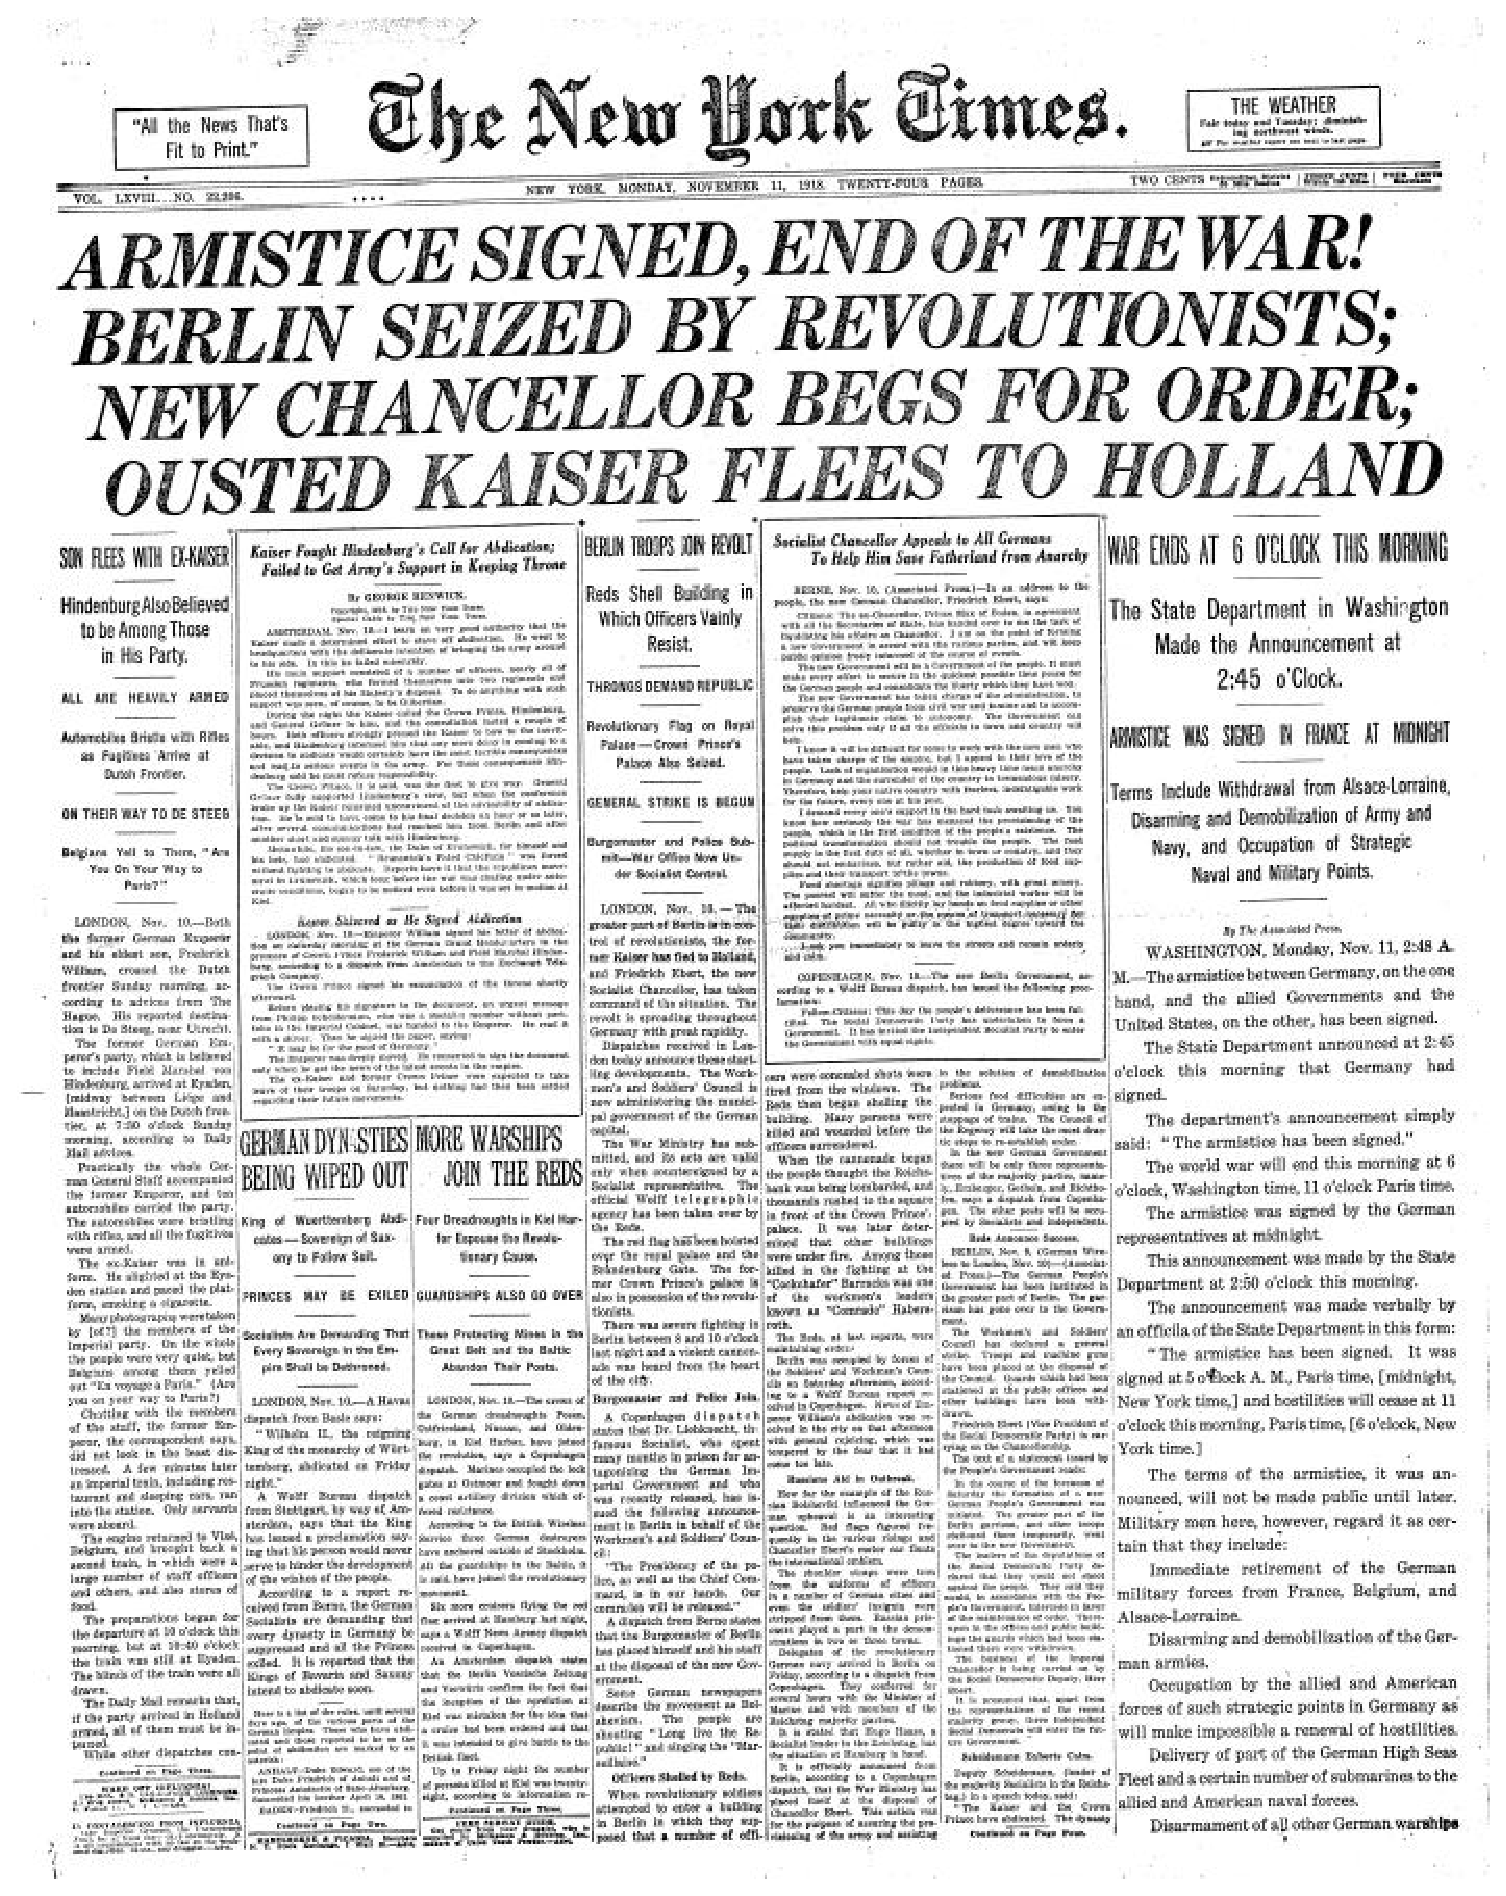
\epsfig{file=figures/times.eps,width=\textwidth}
    \end{minipage}
  \end{tabular}
\end{bbawslide}

\begin{bbawpart}{\Large\bf Workflowbeschreibung}
\end{bbawpart}

\begin{bbawslide}{Übersicht}
  \vspace*{7mm}%
  \centerslidestrue%
  \begin{itemize}
    \item Ziel: Definition und Implementierung eines Workflows
    \begin{itemize}\small
      \item möglichst \textbf{Open Source}
      \item möglichst ohne Programmierkenntnisse einsetzbar
      \item \textbf{lokal} installierbar 
      \item Textergebnis als \textbf{Grundlage einer Edition} verwendbar
    \end{itemize}
    \item Komponenten
    \begin{itemize}\small
      \item Bildvorverarbeitung
      \item Layoutanalyse
      \item Zeichenerkennung
      \item Textbearbeitung
    \end{itemize}
  \end{itemize}
\end{bbawslide}

\begin{bbawslide}{Übersicht}
  \vspace*{2mm}%
  \begin{center}
      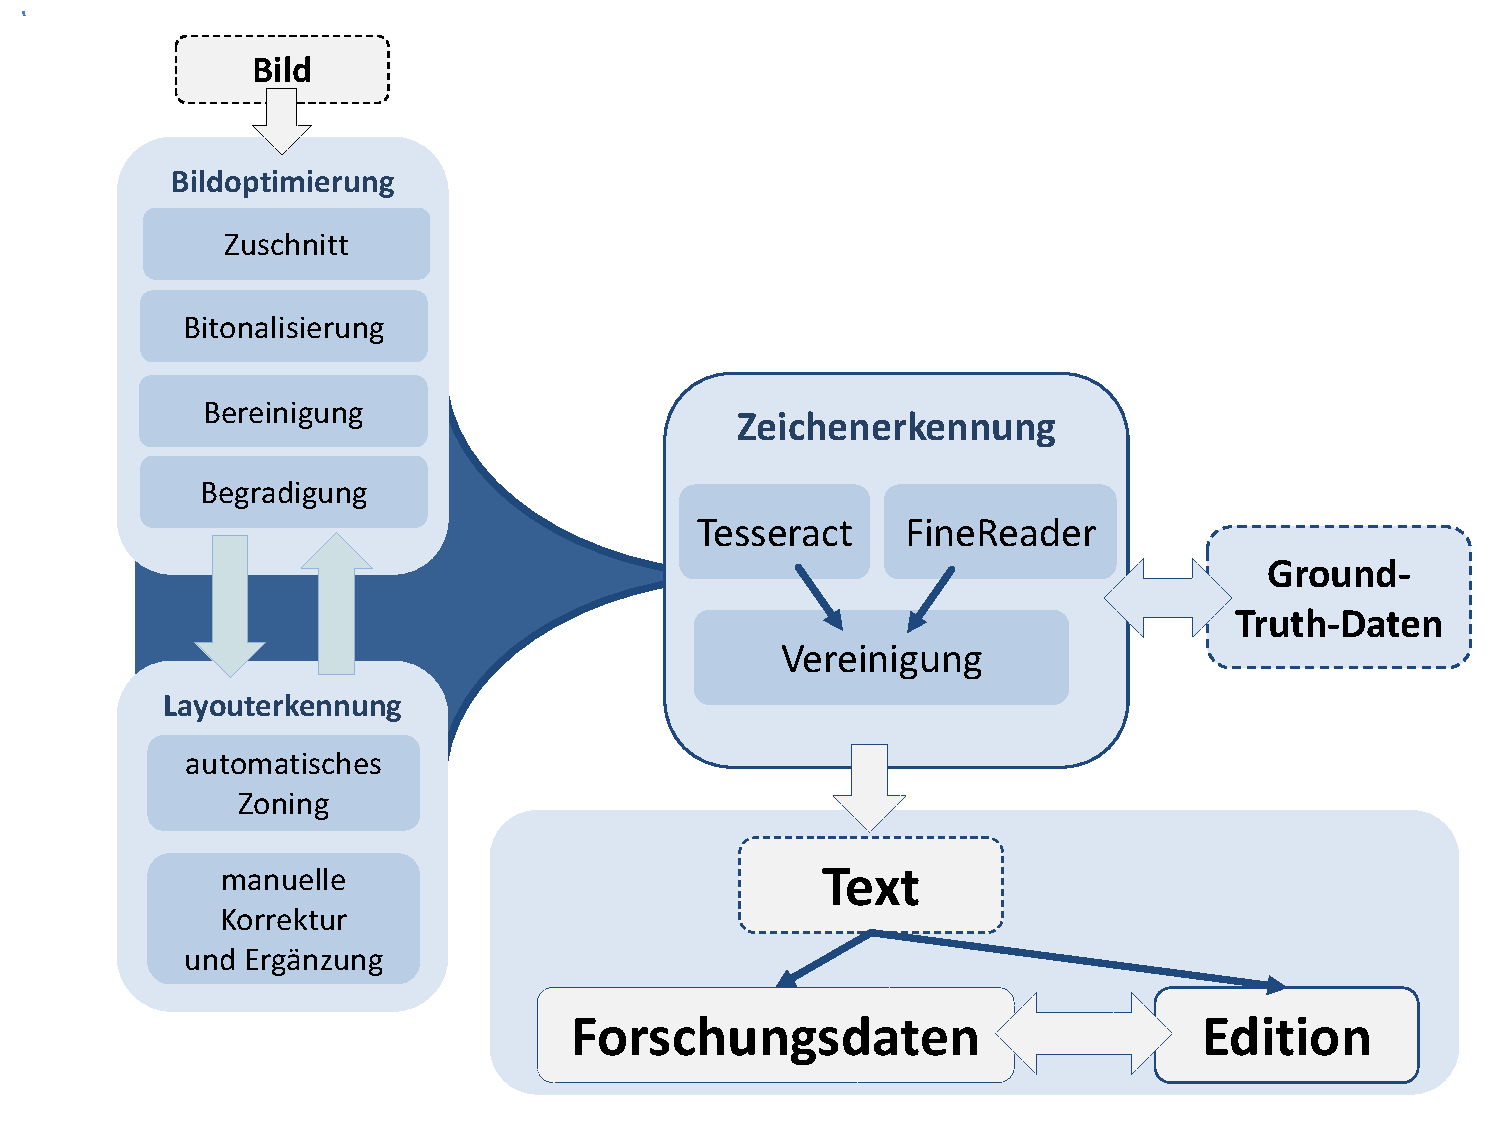
\epsfig{file=figures/workflow.eps,height=\textheight}%
  \end{center}
\end{bbawslide}

\begin{bbawslide}{Bildvorverarbeitung}
  \vspace*{7mm}%
  \centerslidestrue%
  \begin{itemize}
    \item Prozesse zur bestmöglichen Vorbereitung der Digitalisate für OLR und OCR
    \begin{itemize}\small
      \item \textbf{Cropping:} Beschneidung des Digitalisats auf den Druckbereich
      \item \textbf{Deskewing:} Rotation des Digitalisats zur Begradigung von Schrägstellungen
      \item \textbf{Binarization:} Binäre Kodierung der Pixel (bedruckte Bereiche schwarz, nicht-bedruckte Bereiche weiß)
      \item \textbf{Despeckling:} Entfernung von Bildartefakten (Verschmutzungen, sichtbare Papiermaserung etc.)
      \item \textbf{Dewarping:} Begradigung von Wellen auf Zeilenebene
    \end{itemize}
    \item starker Einfluss auf die Erkennungsqualität
    \item besondere Relevanz für historische Vorlagen
  \end{itemize}
\end{bbawslide}

\begin{bbawslide}{Bildvorverarbeitung: ScanTailor}
  \vspace*{7mm}%
  \centerslidestrue%
  \begin{itemize}
    \item umfassendes, frei verfügbares Werkzeug\\
          \url{https://github.com/scantailor/scantailor}
    \begin{description}\small
      \item[+] graphische Benutzerschnittstelle (GUI)
      \item[+] Kommandozeileninterface (CLI)
      \item[-] keine Programmierschnittstelle (API)
    \end{description}
    \item weitgehend \textbf{automatisiert}
    \item erlaubt Stapelverarbeitung
    \item manuelle Korrektur möglich
  \end{itemize}
\end{bbawslide}

\begin{bbawslide}{Bildvorverarbeitung: ScanTailor}
  \vspace*{2mm}%
  \begin{center}
      \epsfig{file=figures/scantailor_screen.eps,height=\textheight}%
  \end{center}
\end{bbawslide}

\begin{bbawslide}{Layoutanalyse}
  \vspace*{7mm}%
  \centerslidestrue%
  \begin{itemize}
    \item Prozesse zur Erkennung der Struktur auf Seiten- und Dokumentebene
    \begin{itemize}\small
      \item \textbf{Page Segmentation:} Lokalisierung von zusammenhängenden Text- und Nichttextbereichen
      \item \textbf{Region Classification:} Typisierung von Textbereichen
      \item \textbf{Line/Character Splitting:} Lokalisierung der einzelnen Zeilen/Zeichen
      \item \textbf{Document Analysis:} Konstruktion der logischen Dokumentstruktur (METS!)
    \end{itemize}
    \item entscheidend für die korrekte \textbf{Rekonstruktion des Textflusses} und damit für maschinelle Auswertungen
  \end{itemize}
\end{bbawslide}

\begin{bbawslide}{Layoutanalyse: LAREX}
  \vspace*{7mm}%
  \centerslidestrue%
  \begin{itemize}
    \item umfassendes, frei verfügbares Werkzeug\\
          \url{https://github.com/chreul/LAREX}
    \begin{description}\small
      \item[+] graphische Benutzerschnittstelle (GUI)
      \item[-] Kommandozeileninterface (CLI)
      \item[-] keine Programmierschnittstelle (API)
    \end{description}
   \item teilweise \textbf{automatisiert}
    \item erlaubt Stapelverarbeitung
    \item manuelle Korrektur \textbf{nötig}
  \end{itemize}
\end{bbawslide}

\begin{bbawslide}{Bildvorverarbeitung: LAREX}
  \vspace*{2mm}%
  \begin{center}
      \epsfig{file=figures/larex_screen.eps,height=\textheight}%
  \end{center}
\end{bbawslide}

\begin{bbawslide}{Bildvorverarbeitung: LAREX}
  \vspace*{2mm}%
  \begin{center}
      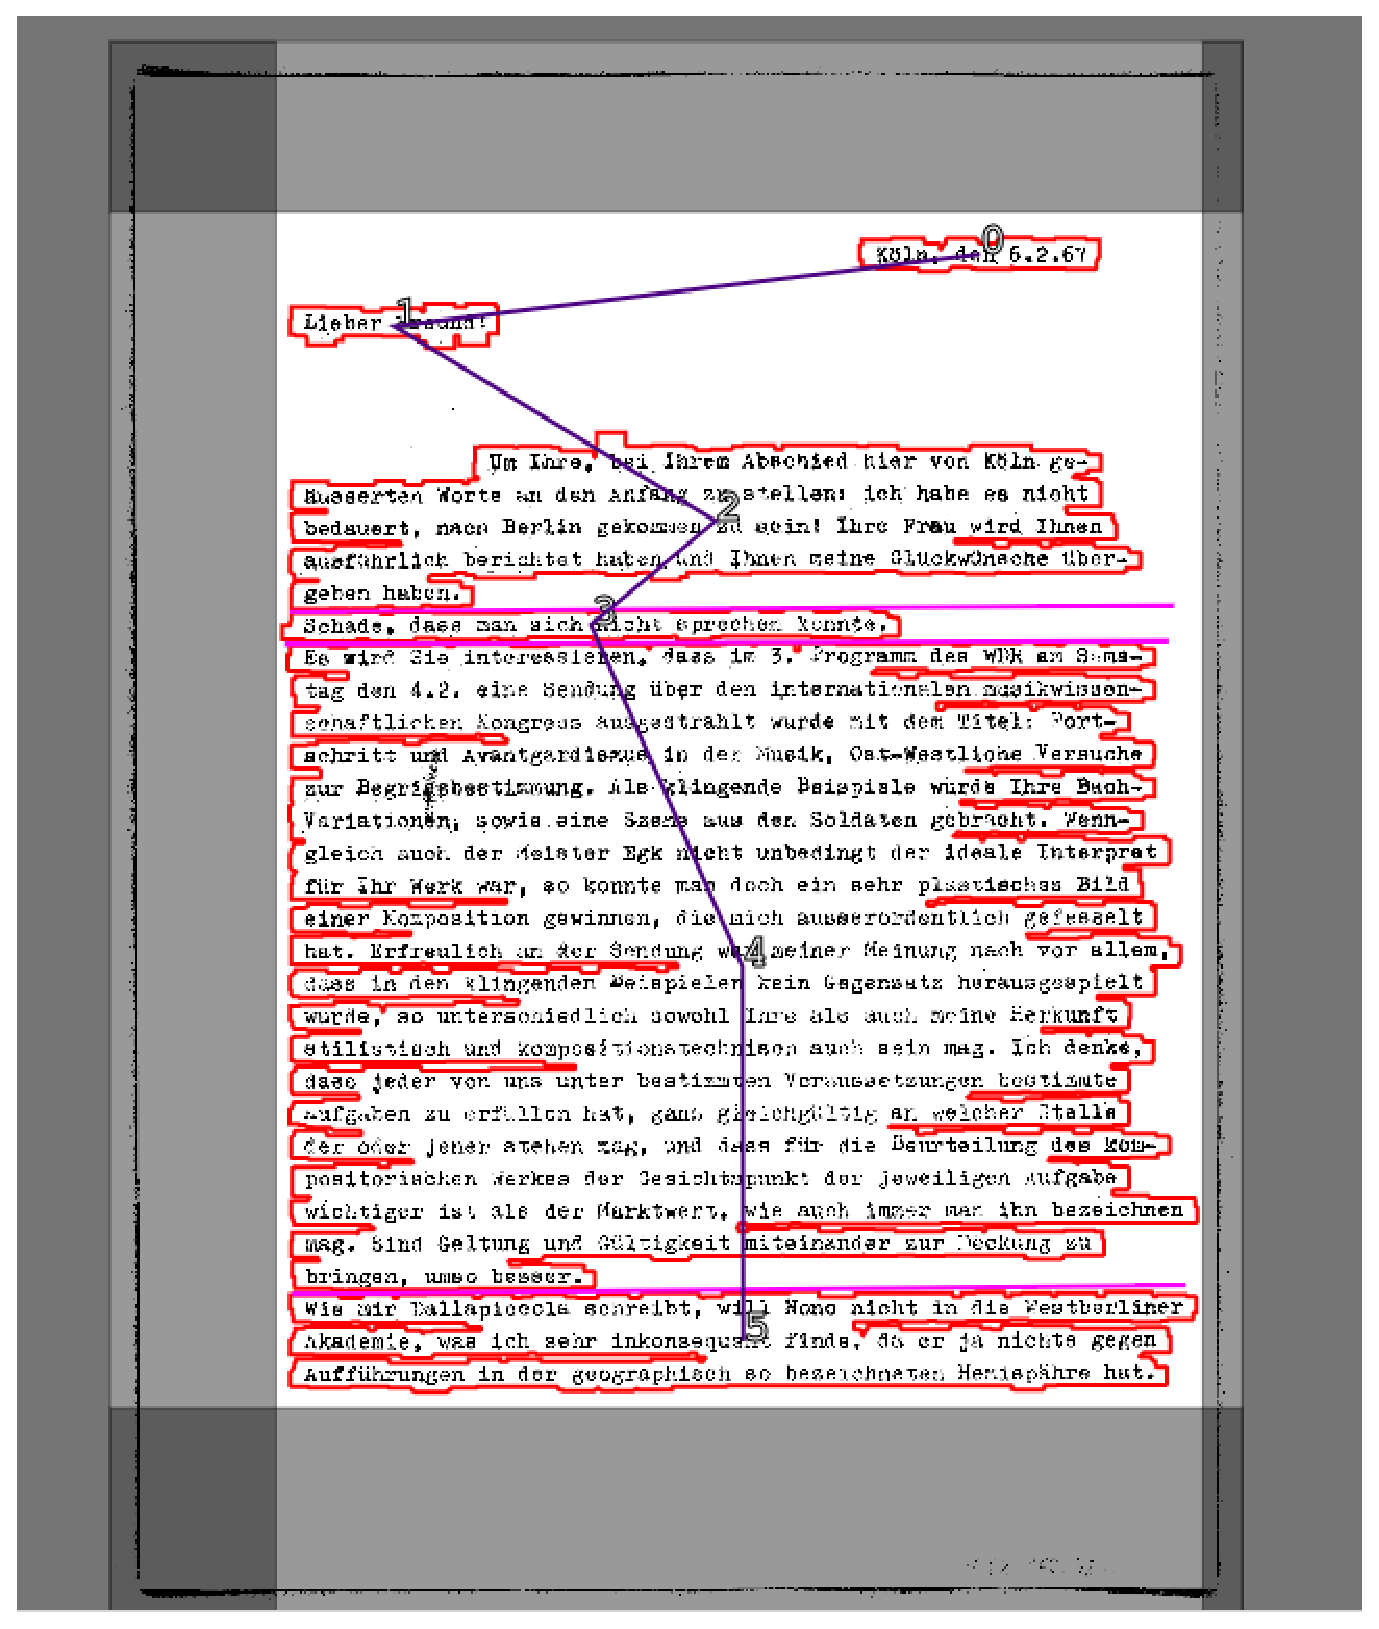
\epsfig{file=figures/larex_result.eps,height=\textheight}%
  \end{center}
\end{bbawslide}

\begin{bbawslide}{Zeichenerkennung}
  \vspace*{7mm}%
  \centerslidestrue%
  \begin{itemize}
    \item Kernkomponente der OCR
    \item Genauigkeit beeinflusst vom Typ des zugrundeliegenden \textbf{Algorithmus} und vom eingesetzten \textbf{Modell}
    \item aktuell Paradigmenwechsel: \textbf{zeichenorientiert} $\rightarrow$ \textbf{zeilenorientiert}
    \begin{itemize} \small
      \item \textbf{Deep learning:} Tiefe (i.e.~vielschichtige) neuronale Netzwerke zur Sequenzklassifizierung \hlcite{Hochreiter und Schmidhuber 1997}
      \item wesentlich weniger anfällig für \textbf{Zeichenvarianz}
      \item eingebautes \textbf{Sprachmodell}
    \end{itemize}
    \item auch schwierige historische Vorlagen in \enquote{OCR-Reichweite} \hlcite{Springmann 2016}
  \end{itemize}
\end{bbawslide}

\begin{bbawslide}{Zeilenorienierte Zeichenerkennung}
  \vspace*{1.5em}%
  \begin{minipage}{1.05\textwidth}
    \begin{itemize}
      \item Bearbeitungsebene sind \textbf{Glyphensequenzen}
      \begin{description}\small
        \item[Skalierung:] einheitliche Höhe für alle Textzeilen
        \item[Merkmalsextraktion:] fixe Anzahl horizontaler Zeilen, variable Anzahl vertikaler Spalten: Textzeilen als binärwertige Vektoren
      \end{description}
    \end{itemize}
  \end{minipage}
  \begin{center}
    
\epsfig{file=figures/grid.eps,width=1.05\textwidth}
  \end{center}
  \begin{minipage}{1.05\textwidth}
    \begin{itemize}
      \item kontextabhängige (i.e.~\emph{Übergangswahrscheinlichkeiten}) Erkennung (größere Mengen an Trainingsmaterial nötig als bei zeichenorientierten Verfahren)
      \item Zeilenerkennung als notwendiger Vorverarbeitungsschritt
      \item Glyphenlokalisierung geschieht en passant
      \item Einsatz neuronaler Netze für den Klassifizierungsschritt
    \end{itemize}
  \end{minipage}
\end{bbawslide}

\begin{bbawslide}{Zeichenerkennung: Textvereinigung}
  \vspace*{7mm}%
  \centerslidestrue%
  \begin{itemize}
    \item Prozesse zur \textbf{Vereinigung} verschiedener OCR-Ergebnisse \textbf{in einen Volltext}
    \item Fehler auch bei \enquote{optimaler} Vorverarbeitung und Verwendung spezifischer Modelle
    \item \textbf{unterschiedliche Engines} bzw. Modelle haben \textbf{unterschiedliche Stärken} und machen unterschiedliche Fehler
    \item Idee: \textbf{Extraktion} korrekt erkannter Textbestandteile \textbf{aus mehreren OCR-Durchgängen} \hlcite{Handley 1998}
    \item Vorteil: Integration vorhandener OCR ebenfalls möglich
    \item \textbf{Reduktion} der Anzahl der falsch erkannten Zeichen\\um 14~\% erzielt \hlcite{Boenig et al. 2016} 
  \end{itemize}
\end{bbawslide}

\begin{bbawslide}{Zeichenerkennung: Werkzeuge}
  \vspace*{7mm}%
  \centerslidestrue%
  \begin{itemize}
    \item ABBYY \texttt{FineReader}
    \begin{itemize}\small
      \item kommerzielle Software, kaum Adaptionsmöglichkeiten
      \item \enquote{Platzhirsch}: großflächiger Einsatz z.B. in Bibliotheken
      \item GUI mit Möglichkeit der Stapelverarbeitung
    \end{itemize}
    \item \texttt{Tesseract} \hlcite{Smith 2007}
    \begin{itemize}\small
      \item Open-Source-Software mit großer Entwicklercommunity
      \item Integration zeilenorientierter Erkennung in Version 4
      \item CLI und API mit weitreichenden Adaptionsmöglichkeiten
    \end{itemize}
    \item \texttt{OCRMerger} \hlcite{Boenig et al. 2016}
    \begin{itemize}\small
      \item Eigenentwicklung
      \item Textvereinigung auf Basis von \texttt{diff}
      \item Konfliktauflösung mit Hilfe von \emph{Ground Truth}
    \end{itemize}
  \end{itemize}
\end{bbawslide}

\begin{bbawslide}{Zeichenerkennung: Ergebnisse}
  \vspace*{7mm}%
  \centerslidestrue%
  Evaluation anhand dreier manuell transkribierter Briefe \\
  \begin{tabular}{lr|lr|lr}
  \multicolumn{2}{r|}{\texttt{FineReader}} & \multicolumn{2}{r|}{\texttt{Tesseract}} & \multicolumn{2}{r}{\texttt{Merged}} \\
  errors    &     302  & & 297 & & 188\\
  missing   &      74  & & 0 & & 0\\
  total     &    5856 & & 5856 & & 5856\\
  err       &   5,157 \% & & 5,072 \% & & 3,210 \% \\
  errnomiss &   3,893 \% & & 5,072 \% & & 3,210 \% \\
  11        &   s	z  & 19 & , . & 9 & , .\\
  10        &   $\neg$	- & 4 & m n & 5 & \_ \\
   6	      &   o	e  & 3 & s \_ & 4 & $\neg$ - \\
   5	      &   «	. & 3 & . \_ & 4 & s z \\
   5	      &   *	. & 3 & z g & 3 & o e \\
  \end{tabular}
  \begin{minipage}{0.2\textwidth}
  \textbf{Reduktion der Zeichenfehler um ca. 37 \%.}
  \end{minipage}
\end{bbawslide}

\begin{bbawslide}{Textbearbeitung}
  \vspace*{7mm}%
  \centerslidestrue%
  \begin{itemize}
     \item kritische \textbf{Textauswahl}
     \item Korrektur und tiefere \textbf{Erschließung}
     \begin{itemize}
       \item Basis: Text-Bild-Ansicht
       \item Auszeichnung von Personen, Orten, Querverweisen etc.
       \item Erläuterungen und Anmerkungen zu spezifischen Sachverhalten und wissenschaftlichen Fragestellungen
     \end{itemize}
     \item Transformation in spezifisches \textbf{Editionsformat}
     \begin{itemize}
       \item Idealfall: nachnutzbares Standardformat (z.B. DTABf)
       \item Normalfall: Verlagsvorgaben
     \end{itemize}
  \end{itemize}
\end{bbawslide}

\begin{bbawslide}{Textbearbeitung: Oxygen}
  \vspace*{7mm}%
  \centerslidestrue%
  \begin{itemize}
    \item kommerzieller \texttt{XML-Editor}
    \begin{itemize}
      \item Marktführer mit großer Verbreitung (vgl. \texttt{ediarum})
      \item weitgehende Anpassungsmöglichkeiten
      \item plattformübergreifend    
    \end{itemize}
    \item \textbf{Unterstützung} des Editionsprozesses durch \textbf{Text-Bild-Ansicht} unter Einbeziehung struktureller Annotationen
    \item \textbf{Operationalisierung} des Editionsprozesses
    \begin{itemize}
      \item spezielle Frameworks
      \item Transformationsszenarien
      \item Einbindung spezieller Schematronregeln
    \end{itemize}
  \end{itemize}
\end{bbawslide}

\begin{bbawslide}{Textbearbeitung: Oxygen}
  \begin{center}
      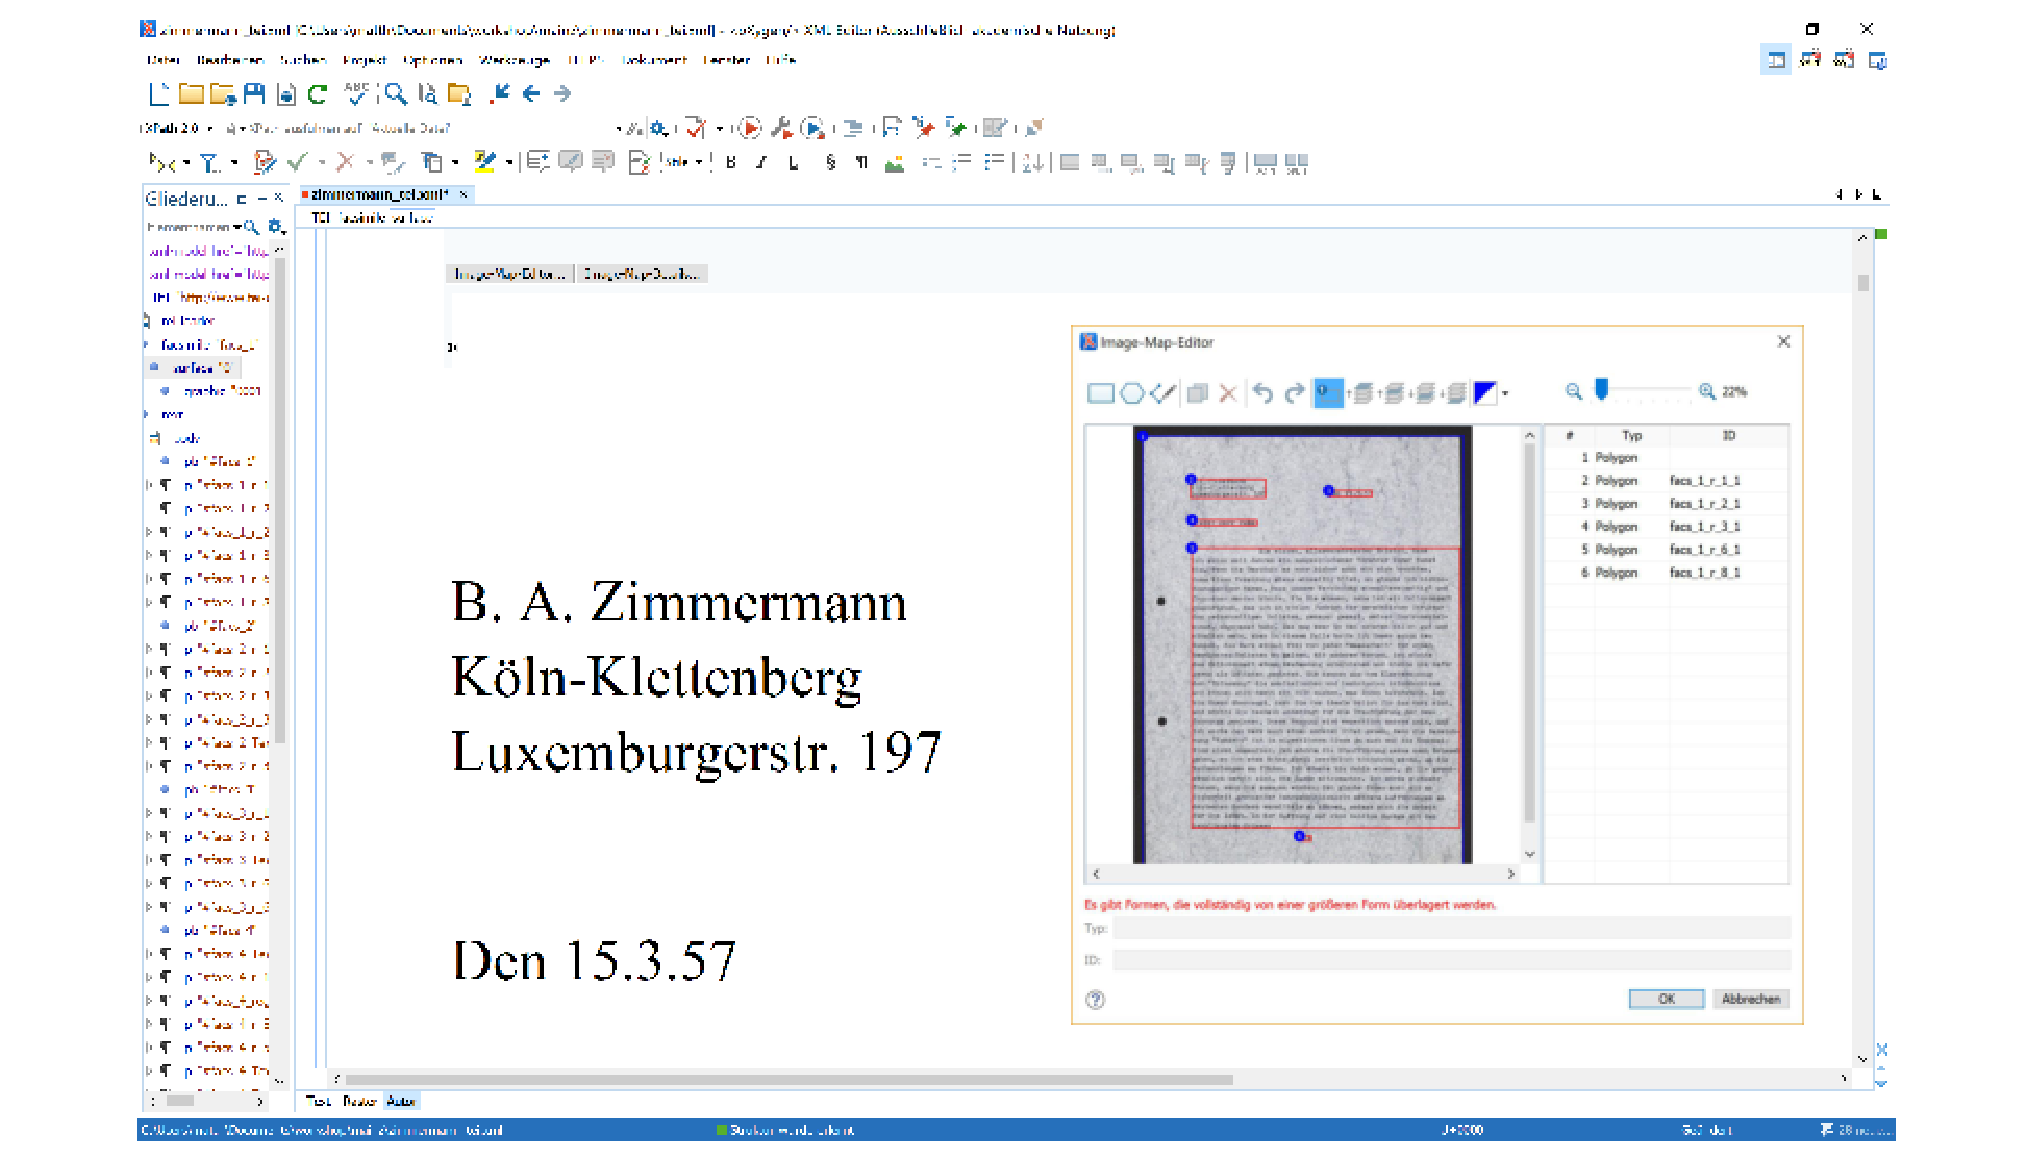
\epsfig{file=figures/oxygen_screen.eps,height=\textheight}%
  \end{center}
\end{bbawslide}

\begin{bbawpart}{\Large\bf Perspektiven}
\end{bbawpart}

\begin{bbawslide}{Volltextverbesserung}
  \vspace*{7mm}%
  \centerslidestrue%
  \begin{itemize}
    \item bisher kein spezifisches Modelltraining
    \begin{itemize}\small
      \item \enquote{echtes} Trainingsmaterial aus manuell erfassten Dokumenten
      \item synthetisches Trainingsmaterial aus Text + Computerfont
    \end{itemize}
    \item bisher kein spezifisches \enquote{Zimmermann-Vokabular}
    \begin{itemize}\small
      \item genauere Zielhypothese bei der Textvereinigung
    \end{itemize}
    \item bisher keine OCR-Nachkorrektur
    \begin{itemize}\small
      \item \texttt{PoCoTo} \hlcite{Vobl et al. 2014}
    \end{itemize}
    \item bisher keine Voting-Verfahren
    \begin{itemize}\small
      \item OCRopus als mögliche weitere OCR-Option \hlcite{Breuel 2008}
    \end{itemize}
  \end{itemize}
\end{bbawslide}

\begin{bbawslide}{OCR-D: Überblick}
  \vspace*{2mm}%
  \centerslidestrue%
  \begin{itemize}
    \item \textbf{DFG-Initiative} zur Verbesserung von OCR-Methoden für historische Drucke, insbesondere
          für die Volltextdigitalisierung aller in den \emph{Verzeichnissen der im deutschen
          Sprachraum erschienen Drucke} (VD16, VD17, VD18) nachgewiesenen Exemplare
    \item \textbf{Koordinationsprojekt} an der Herzog-August Bibliothek Wolfenbüttel, der Staatsbibliothek
          Berlin, dem Karlsruher Institut für Technologie und der BBAW $\rightarrow$ Implementierung
          einer Ausschreibung für methodische
          Projekte auf allen Ebenen eines optimierten OCR-Workflows
    \begin{itemize}\small
      \item Bildvorverarbeitung
      \item Layoutanalyse
      \item Texterkennung/-optimierung
      \item Modelltraining
      \item Langzeitarchivierung
      \item Qualitätssicherung
    \end{itemize}
  \end{itemize}
\end{bbawslide}

\begin{bbawslide}{OCR-D: Projektprämissen}
  \vspace*{7mm}%
  \centerslidestrue%
  \begin{itemize}
    \item \textbf{Lückenschluss} zwischen Forschung und Praxis
    \begin{itemize}\small
      \item Transfer der Forschungsergebnisse
      \item zugängliche und nachnutzbare Implementierungen
    \end{itemize}
    \item \textbf{Methodenpluralismus}
    \begin{itemize}\small
      \item insbesondere bei schwierigen Vorlagen: \textbf{kein} bester Algorithmus
      \item Implementierung möglichst \textbf{vieler Ansätze} samt \enquote{Auswahlmechanismus}
    \end{itemize}
    \item konsequent \textbf{Open Source}
    \begin{itemize}\small
      \item Veröffentlichung des Quellcodes \textbf{und}
      \item Anschluss an vorhandene Communities
    \end{itemize}
  \end{itemize}
\end{bbawslide}

\begin{bbawslide}{Editionsunterstützung}
  \vspace*{1mm}%
  \centerslidestrue%
  \begin{itemize}
    \item Text
    \begin{itemize}\small
      \item Erfassung \textbf{großer Textmengen}
      \item \textbf{kontinuierliche} Erfassung innerhalb des Förderungszeitraums (on Demand)
      \item \textbf{geringe Kosten} nach Einrichtung des Workflows (Modelltraining, Framework)
    \end{itemize}
    \item Forschungsdaten
    \begin{itemize}\small
      \item Erfassung der Primärdaten \textbf{ohne Vorauswahl}
      \item Erschließung der Texte durch \textbf{computerlinguistische Methoden} 
      \item schreibweisentolerante Suche
      \item quantitative Datenanalyse
    \end{itemize}
    \item Edition
    \begin{itemize}\small
      \item Auswahl spezifischer und repräsentativer Korrespondenzbestandteile
      \item \textbf{Aufwertung} durch die große Menge der zur Verfügung stehenden Forschungsdaten
      \item \textbf{Dynamisierung} durch die Möglichkeit der situativen Erweiterung 
    \end{itemize}
  \end{itemize}
\end{bbawslide}

\begin{bbawpart}{\Large\bf Danke für Ihre Aufmerksamkeit!\\}
\end{bbawpart}

\end{document}

%\begin{bbawpart}{\Large\bf Warum braucht man OCR?}
%\end{bbawpart}

%\begin{bbawslide}{Warum braucht man OCR?}
%  \vspace*{7mm}%
%  \centerslidestrue%
%  \begin{itemize}
%    \item
%  \end{itemize}
%\end{bbawslide}

%
% modelines
%

%%% Local Variables:
%%% mode: LaTeX
%%% coding: utf-8
%%% tab-width: 2
%%% indent-tabs-mode: nil
%%% End:

% vim: set ts=2 sw=2 expandtab :
